\section{Aufbau und Durchf"uhrung}
	\label{sec:durchfuehrung}
	\subsection{Bestimmung des effektiven D"ampfungswiderstandes}
		Zun"achst soll die Zeitabh"angigkeit der Amplitude einer ged"ampften Schwingung untersucht und damit der D"ampfungswiderstand bestimmt werden.
		Hierf"ur wird ein Oszilloskop am Kondensator angeschlossen und ein Rechteckpuls in den RLC-Kreis gespeist.
		Der zeitliche Abstand zwischen zwei Pulsen muss gro"s genug gew"ahlt werden, damit eine Abklingen der Amplitude erkennbar ist, bevor die Schwingung neu angeregt wird.
		Der entsprechende Aufbau ist in Abbildung \ref{aufbau_a} zu sehen.

	\subsection{Der D"ampfungswiderstand $R_\mathrm{ap}$ f"ur den aperiodischen Grenzfall}
		Anschlie"send wird der Widerstand $R_\mathrm{ap}$, bei dem der aperiodische Grenzfall eintritt bestimmt.
		Dazu wird der ohmsche Widerstand in Abbildung \ref{aufbau_a} durch einen variablen ersetz und so gro"s gew"ahlt, dass ein reiner Kriechfall vorherrscht.
		Unter beobachtung der Kondensatorspannung $U_\mathrm{C}$ am Oszilloskop wird der Widerstand verkleinert, bis das Signal fast einen Nulldurchgang, bzw. ein "Uberschwingen anzeigt.
		Der Widerstand $R_\mathrm{ap}$ ist dann gefunden.

	\subsection{Frequenzabh"angigkeit der Kondensatorspannung im Serienresonanzkreis}
		Daraufhin speist man die Schaltung mit einer Sinusspannung und misst die Kondensatorspannung $U_\mathrm{C}$ f"ur verschiedene Frequenzen $\omega$.
		Es ist wichtig, dass der Innenwiderstand des Sinusgenerators zum Gesamtwiderstand gerechnet wird.
		Abbildung \ref{aufbau_b} zeigt den entsprechenden Aufbau.

	\subsection{Frequenzabh"angigkeit der Phase zwischen Erreger- und Resonatorfrequenz}
		Schlie"slich wird die Phase in Abh"angigkeit der Frequenz gemessen.
		Dazu wird auch der Sinusgenerator am Oszilloskop angeschlossen und die Nulldurchg"ange bei steigernder Flanke, sowie die Schwingungsdauer beider Signale wie in Abbildung \ref{fig:phase} bestimmt.
		Abbildung \ref{aufbau_c} zeigt den Schaltkreis.
		Es gilt dann

	\begin{equation*}
		\varphi = \frac{a}{b} 2 \pi
	\end{equation*}

	\begin{figure}[h!]
		\centering
		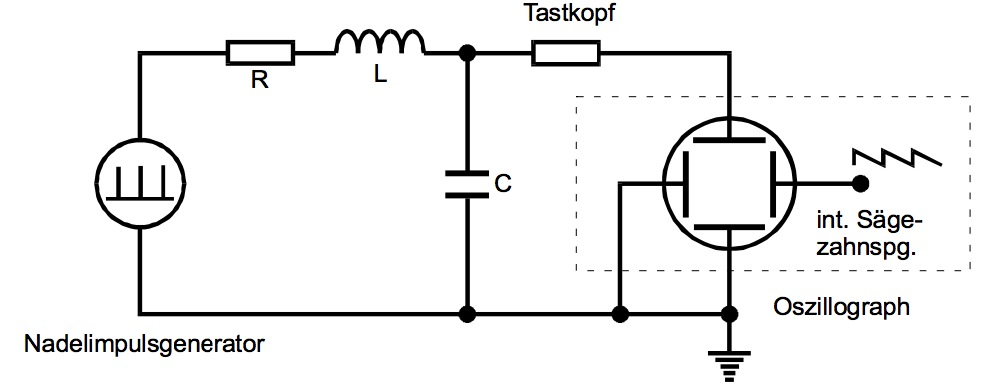
\includegraphics[width = 10cm]{img/aufbaua.JPG}
		\caption{Schaltung f"ur die Bestimmung des D"ampfungswiderstandes. \cite{anleitung}}
		\label{aufbau_a}
	\end{figure}

	\begin{figure}[h!]
		\centering
		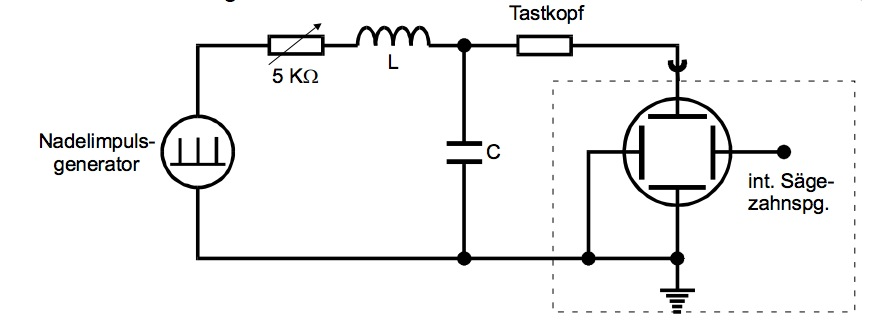
\includegraphics[width = 10cm]{img/aufbaub.JPG}
		\caption{Serienresonanzkreis zur Bestimmung der Frequenzabh"angigkeit der Kondensatorspannung. \cite{anleitung}}
		\label{aufbau_b}
	\end{figure}

	\begin{figure}[h!]
		\centering
		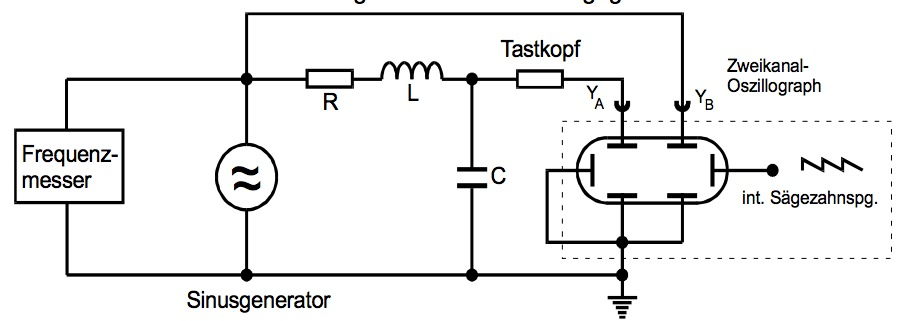
\includegraphics[width = 10cm]{img/aufbauc.JPG}
		\caption{Serienresonanzkreis zur Bestimmung der Frequenzabh"angigkeit der Phase. \cite{anleitung}}
		\label{aufbau_c}
	\end{figure}

	\begin{figure}[h!]
		\centering
		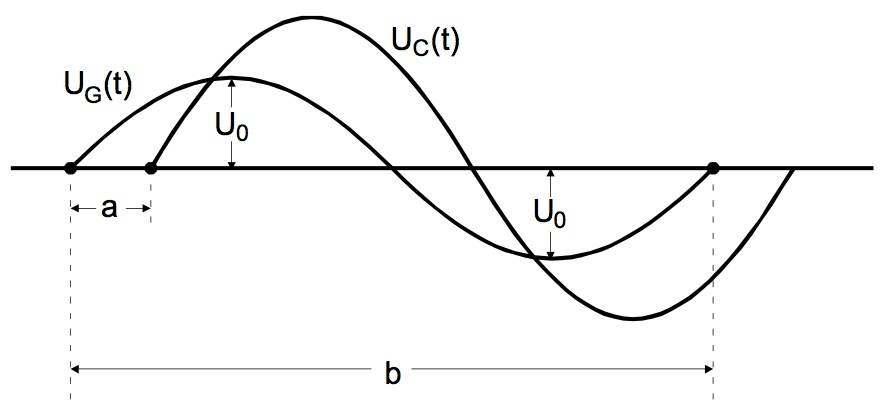
\includegraphics[width = 10cm]{img/phase.JPG}
		\caption{Bestimmung der Phase zweier Sinussignale. \cite{anleitung}}
		\label{fig:phase}
	\end{figure}

	\clearpage